\chapter{Méthodologie et solution proposée}
\label{chap:methode}

\section{Introduction}

Ce chapitre décrit la solution telle qu'elle est codée aujourd'hui : un simulateur en deux dimensions, un catalogue de figures, un contrôleur GNN dont tous les robots partagent les poids, un apprentissage mené à travers la simulation et des protocoles d'évaluation. L'architecture et les valeurs citées sont celles des modules et des fichiers de configuration. Une option présente dans le code ne dit pourtant rien de ce qu'elle donnera après entraînement.

Une règle vaut pour tout le mémoire. Les figures de ce chapitre ne sont pas dessinées à la main : elles viennent du code ou de trajectoires réellement enregistrées par la campagne pilote du chapitre~\ref{chap:experiences}. Ce chapitre s'en sert pour illustrer un mécanisme, pas pour juger un contrôleur. Les résultats, eux, sont discutés au chapitre suivant.

\section{Problème et hypothèses de simulation}

\subsection{Objectif de formation}

Il faut répartir les robots actifs sur une figure, décrite par un ensemble de points de référence, sans attribuer à chaque robot un point précis. Réussir la formation, c'est garder les robots près de la figure, ne laisser aucune partie découverte et éviter les rapprochements dangereux. Les notations utilisées sont réunies dans le Tableau~\ref{tab:notation}.

\begin{table}[htbp]
  \centering
  \caption{Notations utiles à la description de la méthode.}
  \label{tab:notation}
  \begin{tabularx}{\linewidth}{l>{\raggedright\arraybackslash}X}
    \toprule
    Symbole & Signification \\
    \midrule
    $N$, $T$ & nombre de robots et nombre de pas de l'épisode \\
    $p_i^t$, $u_i^t$ & position et commande de vitesse du robot $i$ au pas $t$ \\
    $\Delta t$, $v_{\max}$ & pas de temps et borne de norme de la commande \\
    $r_c$, $\mathcal{N}(i)$ & portée de communication et voisinage du robot $i$ \\
    $h_i^{\ell}$, $m_{ij}^{\ell}$ & état latent et message reçu au tour $\ell$ \\
    $P^t$, $Q$, $R$ & positions des robots actifs, points de référence de la figure et rayon de normalisation \\
    $\theta$, $\tau$ & poids partagés du réseau et seuil de succès \\
    \bottomrule
  \end{tabularx}
\end{table}

\subsection{Dynamique et communication}

L'arène est un carré centré sur l'origine. Le contrôleur produit une commande de vitesse à deux composantes, dont la norme est d'abord plafonnée à $v_{\max}$. La position est alors mise à jour par $p_i^{t+1}=p_i^t+\Delta t\,u_i^t$, puis ramenée sur le bord si elle sort de l'arène. Le modèle reste volontairement simple : vitesse directe, pas d'inertie, ni roues ni contacts mécaniques.

À chaque pas, le graphe est recalculé à partir des distances entre robots. Deux robots actifs sont reliés si leur distance est strictement positive et ne dépasse pas $r_c$ ; un robot n'est pas son propre voisin. Conséquence un peu surprenante, deux robots exactement superposés ne sont pas reliés, alors qu'ils comptent bien dans la mesure de proximité dangereuse. Les échanges passent uniquement par ce graphe, dont la Figure~\ref{fig:communication-graph} du chapitre~\ref{chap:concept} montre deux états réels. Avec une portée de 1,5 dans une arène de côté 4, un robot a souvent plus de la moitié de l'essaim dans son voisinage. Le graphe est donc dense, et ce détail compte pour lire l'effet des messages.

En conditions nominales, les robots partagent un repère commun, observent sans erreur et échangent de façon synchrone. Dans les scénarios de retrait, un robot défaillant reste immobile à sa dernière position enregistrée, mais il sort du graphe, des commandes actives et des métriques. Il ne sert pas d'obstacle. Les perturbations relèvent d'études séparées, distinctes de l'entraînement nominal. Le déroulement différentiable qui sert à apprendre ne contient aucun retrait de robots.

\section{Cibles et information réellement disponible}

\subsection{Représentation et échantillonnage}

La configuration définit sept géométries, dix chiffres, 26 lettres et 21 nombres, soit 64 figures. Une figure est désignée par son nom, \texttt{letters\_A} par exemple, et rien d'autre. On demande aux robots de la dessiner. Pour mesurer s'ils y parviennent, chaque figure est rendue sur une grille de $128\times128$ pixels, puis un échantillonnage par point le plus éloigné retient 50 pixels du trait, tous distincts. Ces 50 points de référence sont les mêmes dans tout le projet, à l'entraînement comme à l'évaluation. Une cible n'est jamais complétée avec des doublons, et un masque trop pauvre est refusé. La méthode répartit bien les points. Elle n'assure en revanche ni une densité régulière le long du trait, ni la conservation de chaque détail.

On recentre ensuite les points sur leur centroïde et on les met à l'échelle pour que leur rayon maximal soit $R=1$. Les distances deviennent sans dimension. Cette échelle commune ne rend pas pour autant les formes également difficiles, ni leurs traits également longs. La Figure~\ref{fig:reference-points} montre le résultat pour six figures, tel que le produit le code du catalogue. On le voit sur le 8 et sur la lettre A : un glyphe a un trait épais, et les points tombent alors dans ce trait, pas seulement sur son contour extérieur.

\begin{figure}[htbp]
  \centering
  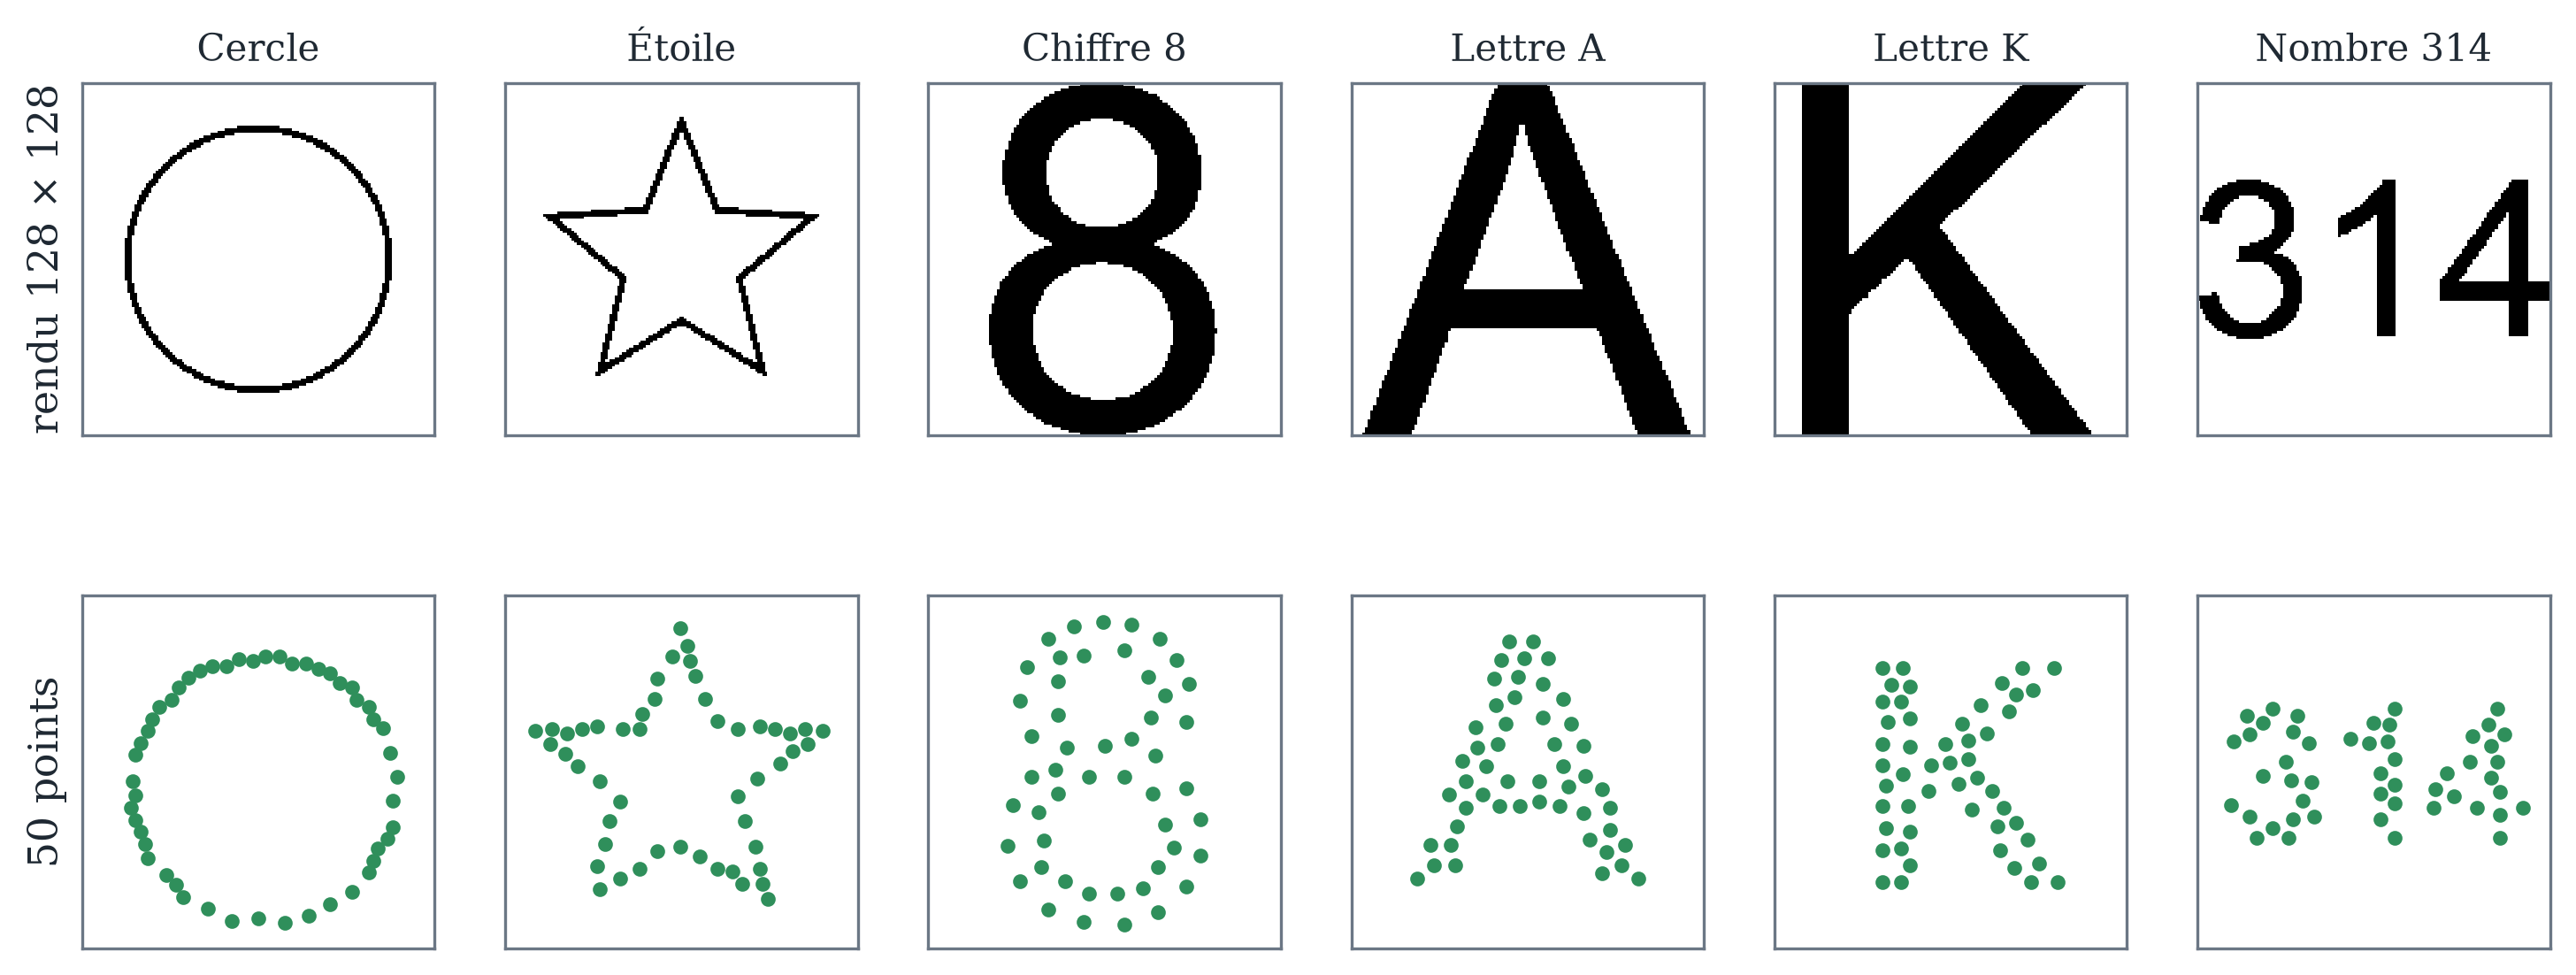
\includegraphics[width=\linewidth,height=.82\textheight,keepaspectratio]{images/real_reference_points.png}
  \caption[Rendu et points de référence de six figures]{Pour six figures du catalogue : rendu binaire $128\times128$ (rangées 1 et 3) et 50 points de référence normalisés (rangées 2 et 4). Images produites par \texttt{src/shapes/}, sans retouche.}
  \label{fig:reference-points}
\end{figure}

Avant tout apprentissage, les figures sont partagées entre entraînement, validation et test, avec respectivement 44, neuf et onze figures. Le nombre 9 est rangé en test, avec le chiffre 9 : c'est le même glyphe, et le placer en entraînement aurait laissé fuir une forme de test. Les figures de test n'interviennent ni dans la mise à jour des poids, ni dans le choix du meilleur modèle. Qu'une forme soit dans le catalogue ne veut pas dire que le modèle l'a vue.

\subsection{Identifiant et direction géométrique}

Le réseau reçoit la vitesse précédente du robot et un plongement appris, de dimension 16, de l'identifiant de figure. La variante géométrique y ajoute deux composantes : la direction \emph{unitaire} vers le point de référence le plus proche. Les points de référence jouent le rôle d'une carte de mission commune, que chaque robot consulte depuis sa position. Cette variante ne reçoit pas la distance au point, seulement sa direction. Sur le point lui-même, la direction calculée est nulle.

La règle manuelle, elle, utilise le déplacement complet vers le point de référence, longueur comprise. Comparer cette règle au GNN ne se fait donc pas à information strictement égale. L'ablation principale oppose plutôt les variantes neuronales avec et sans messages, qui gardent la même consigne géométrique.

La variante à identifiant seul ne reçoit ni position absolue ni direction vers la figure. Rien ne lui indique où se trouve la figure dans l'arène : elle ne dispose que des vitesses, des positions relatives de ses voisins et de l'identifiant. Elle ne peut donc placer la figure au bon endroit que si le centre de l'essaim, au départ, coïncide avec celui de la figure. Elle sert à mesurer ce que la consigne géométrique apporte.

Quand nous parlons de localité, nous parlons des robots dont dépend la commande d'un robot donné. Le programme calcule tout dans un simulateur unique, mais les messages des robots non voisins sont masqués. Une exécution locale est donc possible en principe. Cela reste loin d'un déploiement distribué sur du matériel ou un réseau radio.

\section{Architecture du contrôleur GNN}

\subsection{Encodage et tours de messages}

Chaque robot porte un état caché de 64 composantes. Avec la géométrie, l'entrée compte 20 dimensions (deux pour la vitesse, deux pour la direction, 16 pour l'identifiant) ; sans la géométrie, elle en compte 18. Une transformation affine suivie d'une ReLU donne l'état initial de chaque robot.

À chaque tour, on calcule un message à partir des états des deux robots concernés et de leur position relative, puis on moyenne les messages reçus. L'Équation~\eqref{eq:local-message-aggregation} décrit cette opération, qui fixe à la fois la localité et le traitement d'un nombre variable de voisins :
\begin{equation}
  m_{ij}^{\ell}=\phi_{\ell}(h_i^{\ell},h_j^{\ell},p_j-p_i),
  \qquad
  \bar m_i^{\ell}=\frac{1}{|\mathcal{N}(i)|}\sum_{j\in\mathcal{N}(i)}m_{ij}^{\ell}.
  \label{eq:local-message-aggregation}
\end{equation}
Un voisinage vide donne un agrégat nul. La mise à jour ajoute à l'état précédent une correction apprise, $h_i^{\ell+1}=h_i^{\ell}+\psi_{\ell}(h_i^{\ell},\bar m_i^{\ell})$ : c'est une connexion résiduelle. Les fonctions de message et de mise à jour comprennent chacune deux transformations affines séparées par une ReLU. Les paramètres sont communs à tous les robots, mais chaque tour a les siens.

La configuration nominale prend deux tours, et les variantes préparées en prennent un, deux ou trois. Un tour n'est pas une simple couche, car il combine plusieurs transformations et une agrégation. Sur un graphe fixé pendant le calcul, $L$ tours donnent accès aux informations situées à $L$ sauts au plus. D'un pas de simulation au suivant, les déplacements et les vitesses mémorisées peuvent en plus faire circuler une influence plus ancienne.

Le Tableau~\ref{tab:gnn-layers} détaille les couches du modèle à deux tours, telles que les affiche PyTorch. On compte onze couches linéaires et une table de plongement des figures, dans le cadre général du passage de messages \cite{gilmer2017}. Chaque tour ajoute quatre couches, si bien que les variantes à un, deux et trois tours ont 31\,618, 56\,578 et 81\,538 paramètres. Ce nombre ne dépend pas de l'effectif, puisque tous les robots partagent les mêmes poids.

\begin{table}[htbp]
  \centering
  \small
  \caption{Couches du GNN à deux tours avec direction géométrique (56\,578 paramètres).}
  \label{tab:gnn-layers}
  \begin{tabularx}{\linewidth}{>{\raggedright\arraybackslash}p{.27\linewidth}>{\raggedright\arraybackslash}p{.27\linewidth}>{\raggedright\arraybackslash}X}
    \toprule
    Bloc & Couches & Dimensions \\
    \midrule
    Encodeur & plongement + 1 linéaire & identifiant $\to$ 16 ; $2+2+16=20 \to 64$ \\
    Tour 1 : message & 2 linéaires & $64+64+2=130 \to 64 \to 64$ \\
    Tour 1 : mise à jour & 2 linéaires & $64+64=128 \to 64 \to 64$ \\
    Tour 2 & 4 linéaires & identiques, poids propres \\
    Décodeur & 2 linéaires & $64 \to 64 \to 2$, puis tangente hyperbolique et bornage \\
    \bottomrule
  \end{tabularx}
\end{table}

\subsection{Sortie bornée et propriétés structurelles}

Le décodeur transforme l'état final en deux composantes, leur applique une tangente hyperbolique, les multiplie par $v_{\max}$, puis projette radialement la commande dans le disque de rayon $v_{\max}$ si elle en sort. Dans la variante géométrique, la direction unitaire vers le point de référence le plus proche est d'abord ajoutée aux deux composantes issues du réseau, avant la tangente hyperbolique, avec un poids de 1 par défaut. Avant tout apprentissage, la commande pointe donc déjà, pour une large part, vers la figure ; le réseau apprend une correction autour de cette direction. Le bornage tient toujours. Ce poids est un choix de conception, pas un résultat ; à zéro, le décodeur redevient purement appris. La tangente hyperbolique borne chaque composante séparément, et c'est la projection qui garantit la borne euclidienne. Quant à la ReLU des couches internes, elle ne joue aucun rôle de sécurité.

L'agrégat ne dépend pas de l'ordre des voisins, et le contrôleur est \emph{équivariant} par permutation des robots : si l'on renumérote les robots, les commandes sont renumérotées de la même façon. Translater toutes les positions ne change pas les positions relatives, donc pas les messages. Dans la variante géométrique, il faut cependant translater les robots et la figure ensemble, hors effets de bord. Déplacer les robots seuls devant une figure fixe modifierait la commande. Nous ne revendiquons aucune invariance générale par rotation.

La variante sans communication garde le modèle à deux tours et le même nombre de paramètres, mais fonctionne sur un graphe vide. Les agrégats sont nuls, tandis que les transformations locales et les connexions résiduelles restent actives. Ce n'est donc pas un réseau sans couches de messages. L'ablation isole l'effet des échanges sans retirer de paramètres en même temps.

\section{Apprentissage et fonction de perte}

\subsection{Proximité et couverture : deux directions distinctes}

La distance de Chamfer compare deux ensembles sans imposer de bijection. Pour les positions actives $P$ et la cible $Q$, l'Équation~\eqref{eq:chamfer} donne la mesure utilisée par l'évaluation actuelle, avec des distances euclidiennes \emph{non carrées} :
\begin{equation}
  d_C(P,Q)=\frac{1}{R}\left[
  \frac{1}{|P|}\sum_{p\in P}\min_{q\in Q}\lVert p-q\rVert+
  \frac{1}{|Q|}\sum_{q\in Q}\min_{p\in P}\lVert q-p\rVert\right].
  \label{eq:chamfer}
\end{equation}
Le premier terme mesure la proximité : la distance moyenne de chaque robot à la figure. Le second mesure la couverture. Une partie de la figure éloignée de tous les robots le fait grimper, même si les robots présents sont tout près d'un petit arc. Plusieurs points de référence peuvent avoir le même robot pour plus proche voisin : la mesure n'impose aucune affectation un à un.

La Figure~\ref{fig:proximity-coverage} sépare les deux termes sur un épisode réel de la règle manuelle, sur l'étoile. La proximité tombe sous 0,01 : chaque robot est posé sur la figure. La couverture, elle, reste vers 0,11, parce que des branches de l'étoile n'ont pas de robot. C'est elle qui décide si l'épisode passe le seuil.

\begin{figure}[htbp]
  \centering
  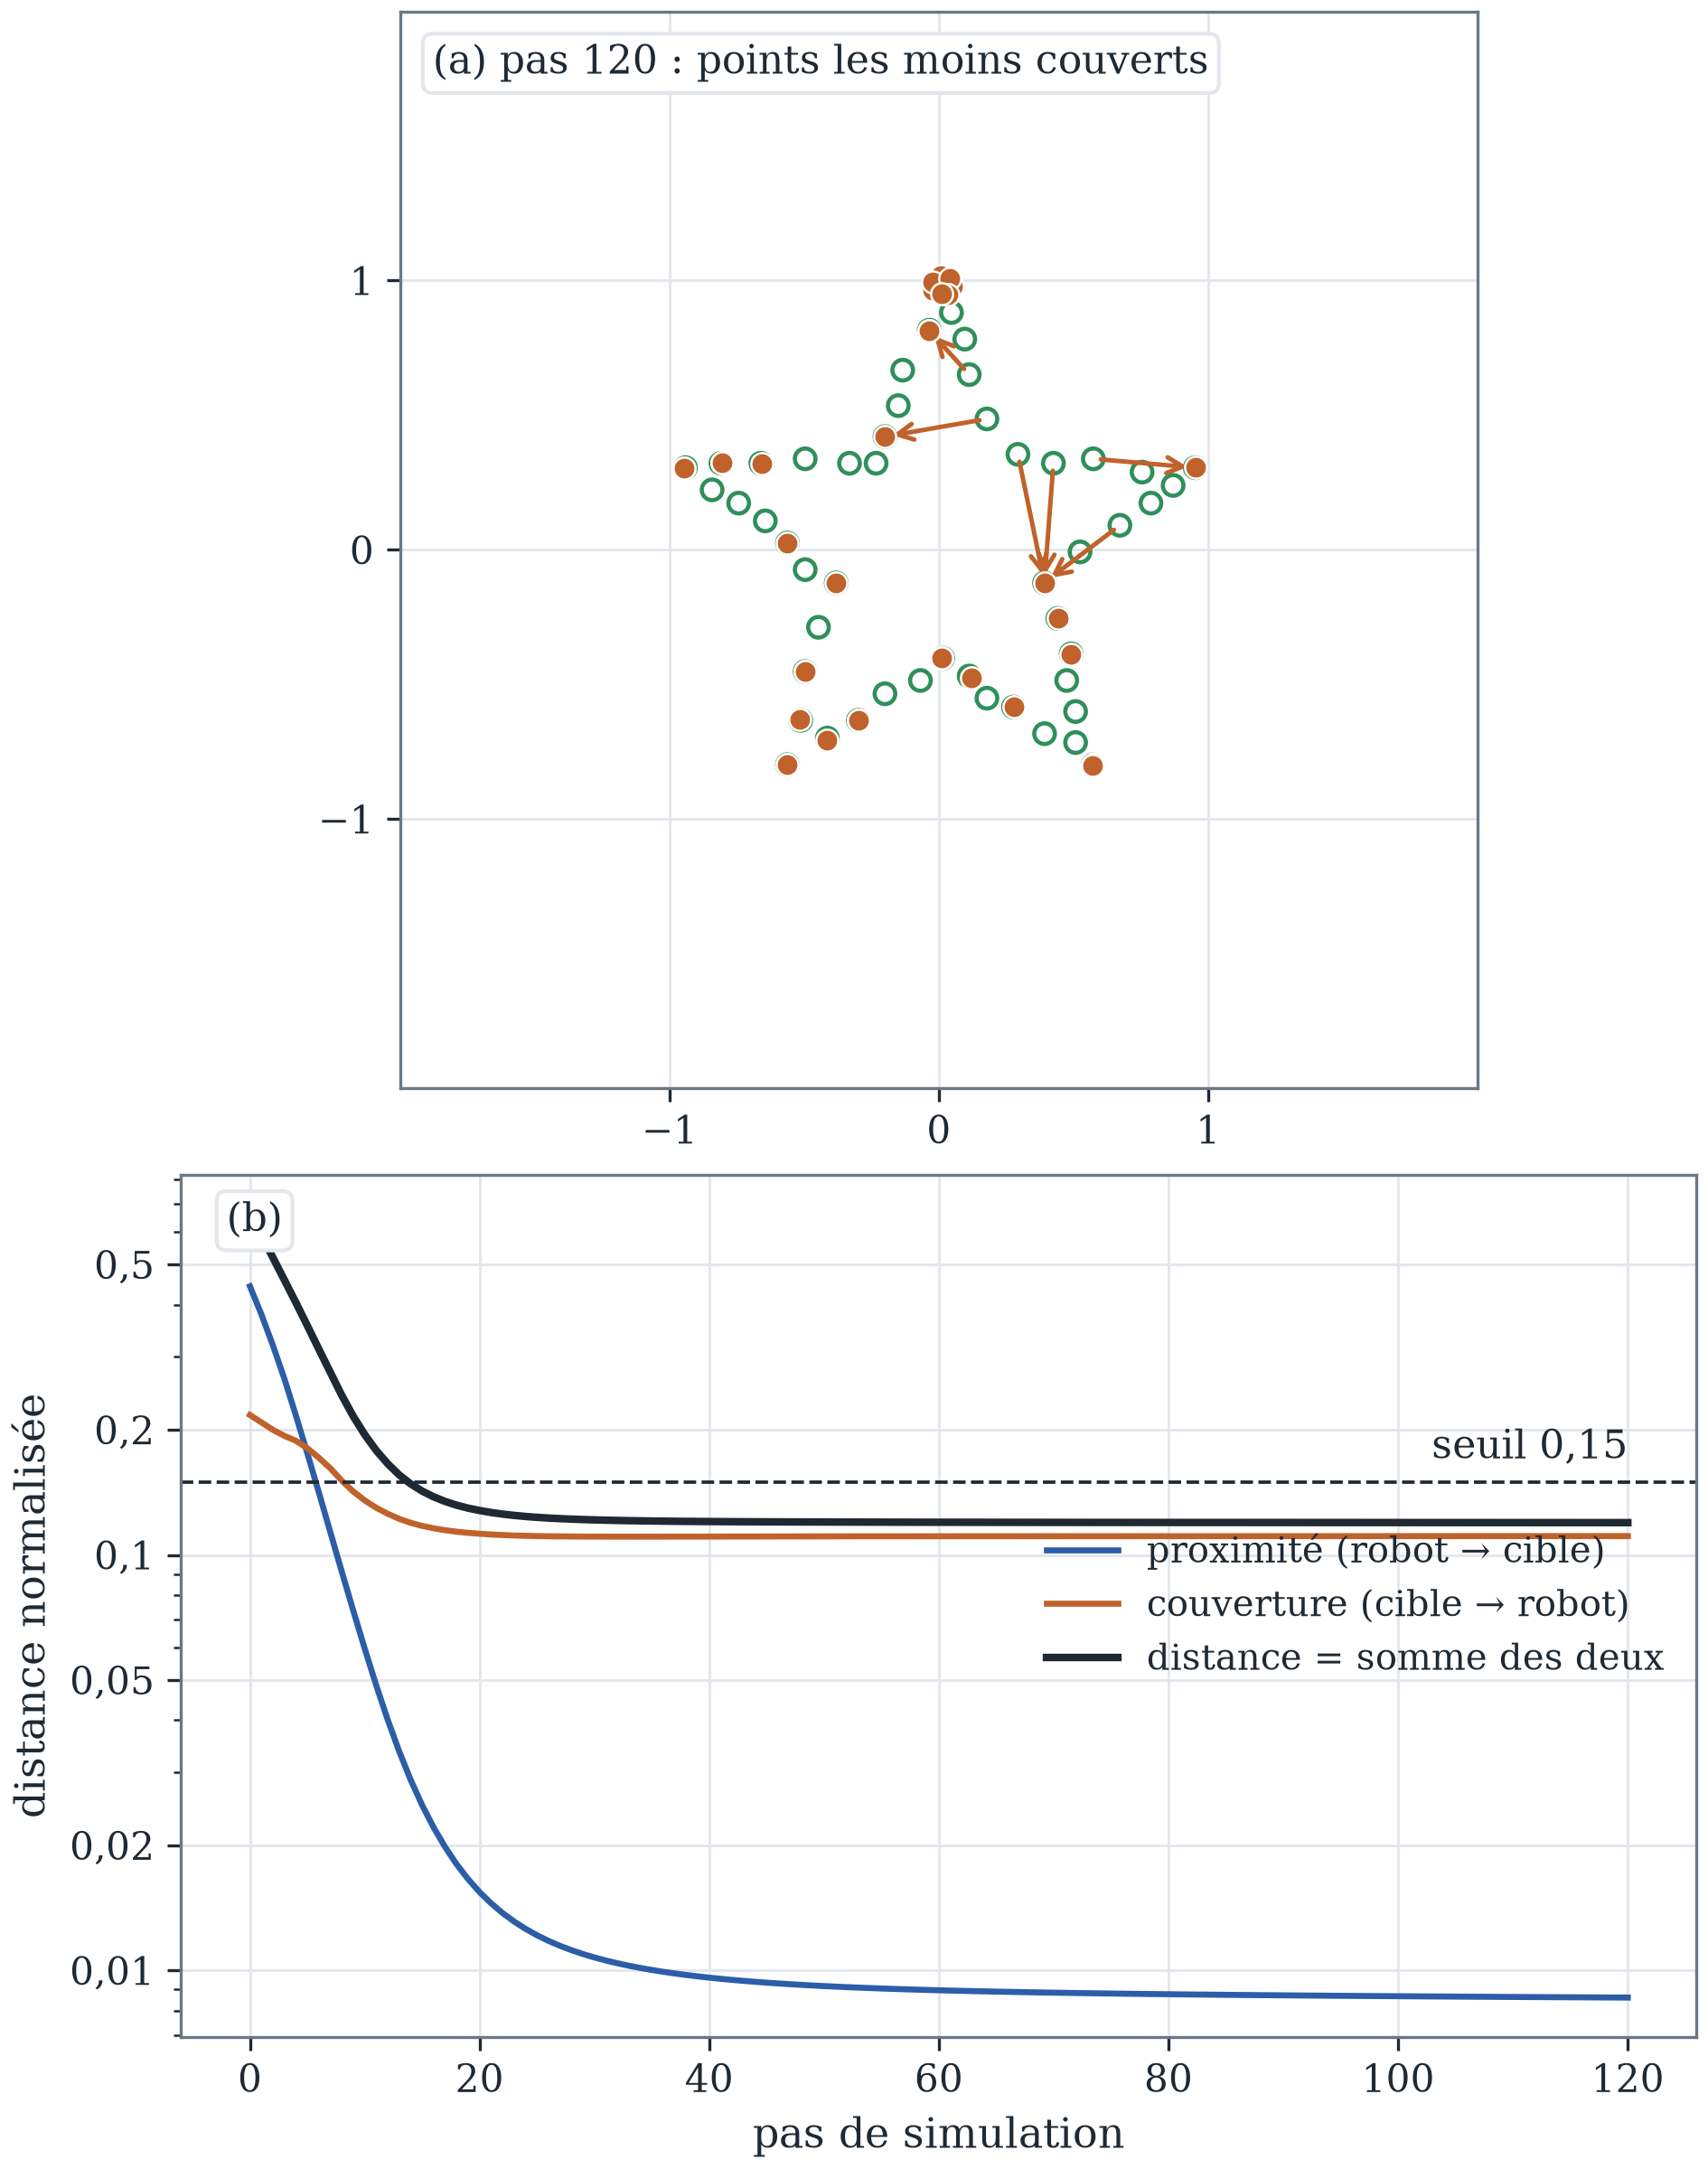
\includegraphics[width=\linewidth,height=.82\textheight,keepaspectratio]{images/real_proximity_coverage.png}
  \caption[Proximité et couverture sur un épisode réel]{Proximité et couverture sur un épisode réel de la règle manuelle (étoile, 40 robots, graine 555000) : (a) état final, les flèches partent des points de référence les moins couverts vers le robot le plus proche ; (b) évolution des deux termes et de leur somme. Positions lues dans \texttt{outputs/evaluation\_pilot/manual/positions/}.}
  \label{fig:proximity-coverage}
\end{figure}

La perte d'entraînement garde ces deux termes séparés, tous deux non quadratiques et normalisés par $R$, chacun avec son propre poids. Dans le profil nominal, on les moyenne sur les dix derniers états de la trajectoire, pas seulement sur l'état final. Le terme de couverture ne compare pas les espacements entre voisins. La Chamfer symétrique pénalise déjà les zones découvertes, sans garantir une distribution uniforme ni la lisibilité d'une lettre.

\subsection{Sécurité et régularisation du mouvement}

L'Équation~\eqref{eq:perte-totale} garde le strict nécessaire pour savoir ce qui est optimisé :
\begin{equation}
  \mathcal{L}=\lambda_f\mathcal{L}_{forme}+\lambda_r\mathcal{L}_{couverture}
  +\lambda_c\mathcal{L}_{collisions}+\lambda_u\mathcal{L}_{mouvement}.
  \label{eq:perte-totale}
\end{equation}
La pénalité de collisions est nulle au-delà de la distance de sécurité et quadratique en deçà, après normalisation par cette distance. On la moyenne sur les paires, puis sur les états, l'état final compris. Sa valeur reste donc entre 0 et 1, quel que soit le nombre de robots. Les dix premiers états sont écartés, car le chevauchement qui sort du tirage initial ne vient d'aucune commande et son gradient ne serait que du bruit.

Ce n'était pas le cas des modèles évalués au chapitre~\ref{chap:experiences}. Leur perte additionnait les pénalités sur toutes les paires, et ce terme valait à lui seul environ 97\,\% de la perte totale en début d'entraînement. Nous l'avons corrigé le 28 octobre 2026, après avoir lu les journaux d'entraînement.

La pénalité de mouvement moyenne la norme carrée des commandes sur tous les pas et tous les robots, divisée par $v_{\max}^2$. Elle décourage les vitesses élevées. Elle ne punit pas explicitement les variations dans le temps, l'accélération ou les oscillations, et elle ne représente pas une énergie physique mesurée. Les poids configurés valent 1 pour la forme, 1 pour la couverture, 0,5 pour les collisions et 0,02 pour le mouvement. Avec la nouvelle perte de collisions, le poids de 0,5 pèse beaucoup moins qu'avant et devra être réglé de nouveau, avec le même budget pour toutes les variantes. Sans ablation, on ne peut affirmer aucun effet causal d'une composante.

\subsection{Déroulement de l'optimisation}

Les poids sont ajustés à partir d'une perte globale calculée sur la simulation, sans commandes d'expert ni récompenses individuelles. Les épisodes d'un lot sont déroulés l'un après l'autre, leurs pertes sont moyennées, puis Adam met à jour les poids. Le meilleur modèle est choisi sur la distance moyenne de validation, pas sur la dernière perte d'entraînement, et le dernier état est gardé à part. Ce choix a compté en pratique : le GNN à trois tours a divergé vers l'itération 700, et c'est son état de l'itération 450 qui a été évalué (Figure~\ref{fig:training-curves}).

PyTorch garde la trace des opérations qui relient positions et commandes aux poids partagés. Deux décisions restent pourtant discrètes, le graphe booléen de voisinage et le choix du point cible le plus proche. Le gradient ne traverse ni l'apparition d'une arête ni le changement d'indice sélectionné. Les ReLU, les minimums et les écrêtages ajoutent des points non lisses ou des zones saturées. La simulation est donc différentiable par morceaux, le long des chemins enregistrés, et non une fonction lisse de toute la topologie.

\section{Configurations actuelles et curriculum}

\subsection{Valeurs de configuration}

Les valeurs du profil standard sont rassemblées dans le Tableau~\ref{tab:hyperparametres}. Ce sont des réglages choisis, pas des valeurs optimisées : rien n'indique qu'elles soient les meilleures. Le simulateur général a un horizon par défaut de 60 pas. Le profil d'entraînement sur le cercle le ramène à 40 et la campagne d'évaluation le porte à 120. Cet écart n'est pas anodin : un modèle n'a jamais été optimisé sur ce qui se passe après le pas 40.

\begin{table}[htbp]
  \centering
  \small
  \caption{Hyperparamètres et réglages de l'entraînement standard et de l'évaluation.}
  \label{tab:hyperparametres}
  \begin{tabularx}{\linewidth}{>{\raggedright\arraybackslash}p{.53\linewidth}>{\raggedright\arraybackslash}X}
    \toprule
    Réglage & Valeur configurée \\
    \midrule
    Arène ; rayon de cible ; rayon de départ & $4\times4$ ; 1 ; 1,8 \\
    Pas de temps ; vitesse maximale & 0,1 ; 1 \\
    Portée ; distance de sécurité & 1,5 ; 0,1 \\
    Robots ; points de référence par figure & 40 ; 50 \\
    Largeur cachée ; représentation de forme & 64 ; 16 \\
    Tours de messages ; agrégation nominale & 1, 2 ou 3 ; moyenne \\
    Horizon cercle ; horizon d'évaluation & 40 ; 120 \\
    Itérations ; épisodes par lot & 1\,200 ; 8 \\
    Taux d'apprentissage initial ; décroissance & 0,001 ; facteur 0,999 par itération \\
    Borne de norme du gradient & 1 \\
    Fenêtre de proximité et de couverture & 10 derniers états \\
    États initiaux exclus des collisions & 10 premiers \\
    Poids de la direction dans le décodeur & 1 \\
    Graines d'entraînement & 11, 12, 13, 14, 15 \\
    Graines de validation & 9001, 9002, 9003 \\
    Validation ; répétitions d'évaluation & toutes les 50 itérations ; 50 par condition \\
    Seuil actuel de succès & 0,15 sur la Chamfer normalisée \\
    \bottomrule
  \end{tabularx}
\end{table}

L'entraînement initial porte sur le cercle. La validation combine de nouveaux départs sur cette cible et une forme du découpage de validation, le pentagone. On retient le meilleur état d'après la moyenne des distances sur les cibles et les graines de validation. Les profils de transfert de taille prévoient séparément 20, 40 et 100 robots. Des modèles entraînés existent pour 20 et pour 40, et celui de 100 robots reste inachevé.

\subsection{Progression cumulative et oubli}

Le curriculum actuel distingue deux variantes à trois tours, l'une avec l'identifiant seul et l'autre avec l'identifiant et la géométrie. Chaque niveau garde les formes des niveaux précédents. Le Tableau~\ref{tab:current-curriculum} donne le nombre de figures à chaque niveau ; ce sont des figures disponibles, pas des figures maîtrisées. Aucun entraînement par curriculum n'a encore été lancé.

\begin{table}[htbp]
  \centering
  \caption{Figures cumulées par niveau du curriculum actuel.}
  \label{tab:current-curriculum}
  \begin{tabular}{lrr}
    \toprule
    Niveau & Cibles d'entraînement & Cibles de validation \\
    \midrule
    Géométries & 5 & 1 \\
    Ajout des chiffres & 11 & 3 \\
    Ajout des lettres & 31 & 6 \\
    Ajout des nombres & 44 & 9 \\
    \bottomrule
  \end{tabular}
\end{table}

Le profil standard prévoit 50 robots, 120 pas et 1\,200 itérations par niveau. Le meilleur état d'un niveau initialise les poids du suivant, après un contrôle de compatibilité. L'empreinte du fichier transféré est calculée, puis notée dans la configuration effective. L'état de l'optimiseur, lui, ne passe pas d'un niveau à l'autre. Les mêmes cibles et graines de validation sont réévaluées pour mesurer la variation de distance. Une hausse supérieure à 0,05 est signalée comme un oubli notable ; cette tolérance est une convention, pas une valeur justifiée. Garder les figures précédentes vise à limiter l'oubli, mais l'efficacité de ce choix reste à mesurer \cite{kirkpatrick2017}.

\section{Évaluation : définition et limites des mesures}

\subsection{Succès et franchissement stabilisé}

La mesure actuelle repose sur la Chamfer normalisée de l'Équation~\eqref{eq:chamfer}. Un épisode est réussi s'il existe un pas à partir duquel toutes les distances enregistrées restent inférieures ou égales à 0,15 jusqu'à la fin. On rapporte le début de ce suffixe. Passer sous le seuil puis le dépasser de nouveau ne suffit donc pas. Si seul l'état final est sous le seuil, le suffixe compte un seul état et l'épisode est accepté. Cette convention ne prouve pas une stabilité durable au-delà de l'horizon observé, et encore moins une convergence asymptotique.

La Figure~\ref{fig:success-criterion} applique cette règle à cinq épisodes réels du GNN à trois tours. Sur le cercle, les courbes descendent vite sous le seuil et y restent ; le point marque le pas retenu. Sur l'étoile, elles se stabilisent juste au-dessus. Aucun de ces cinq épisodes n'est compté comme réussi, alors que leurs distances diffèrent à peine de celles du cercle. Le seuil tranche net là où les distances varient peu.

\begin{figure}[htbp]
  \centering
  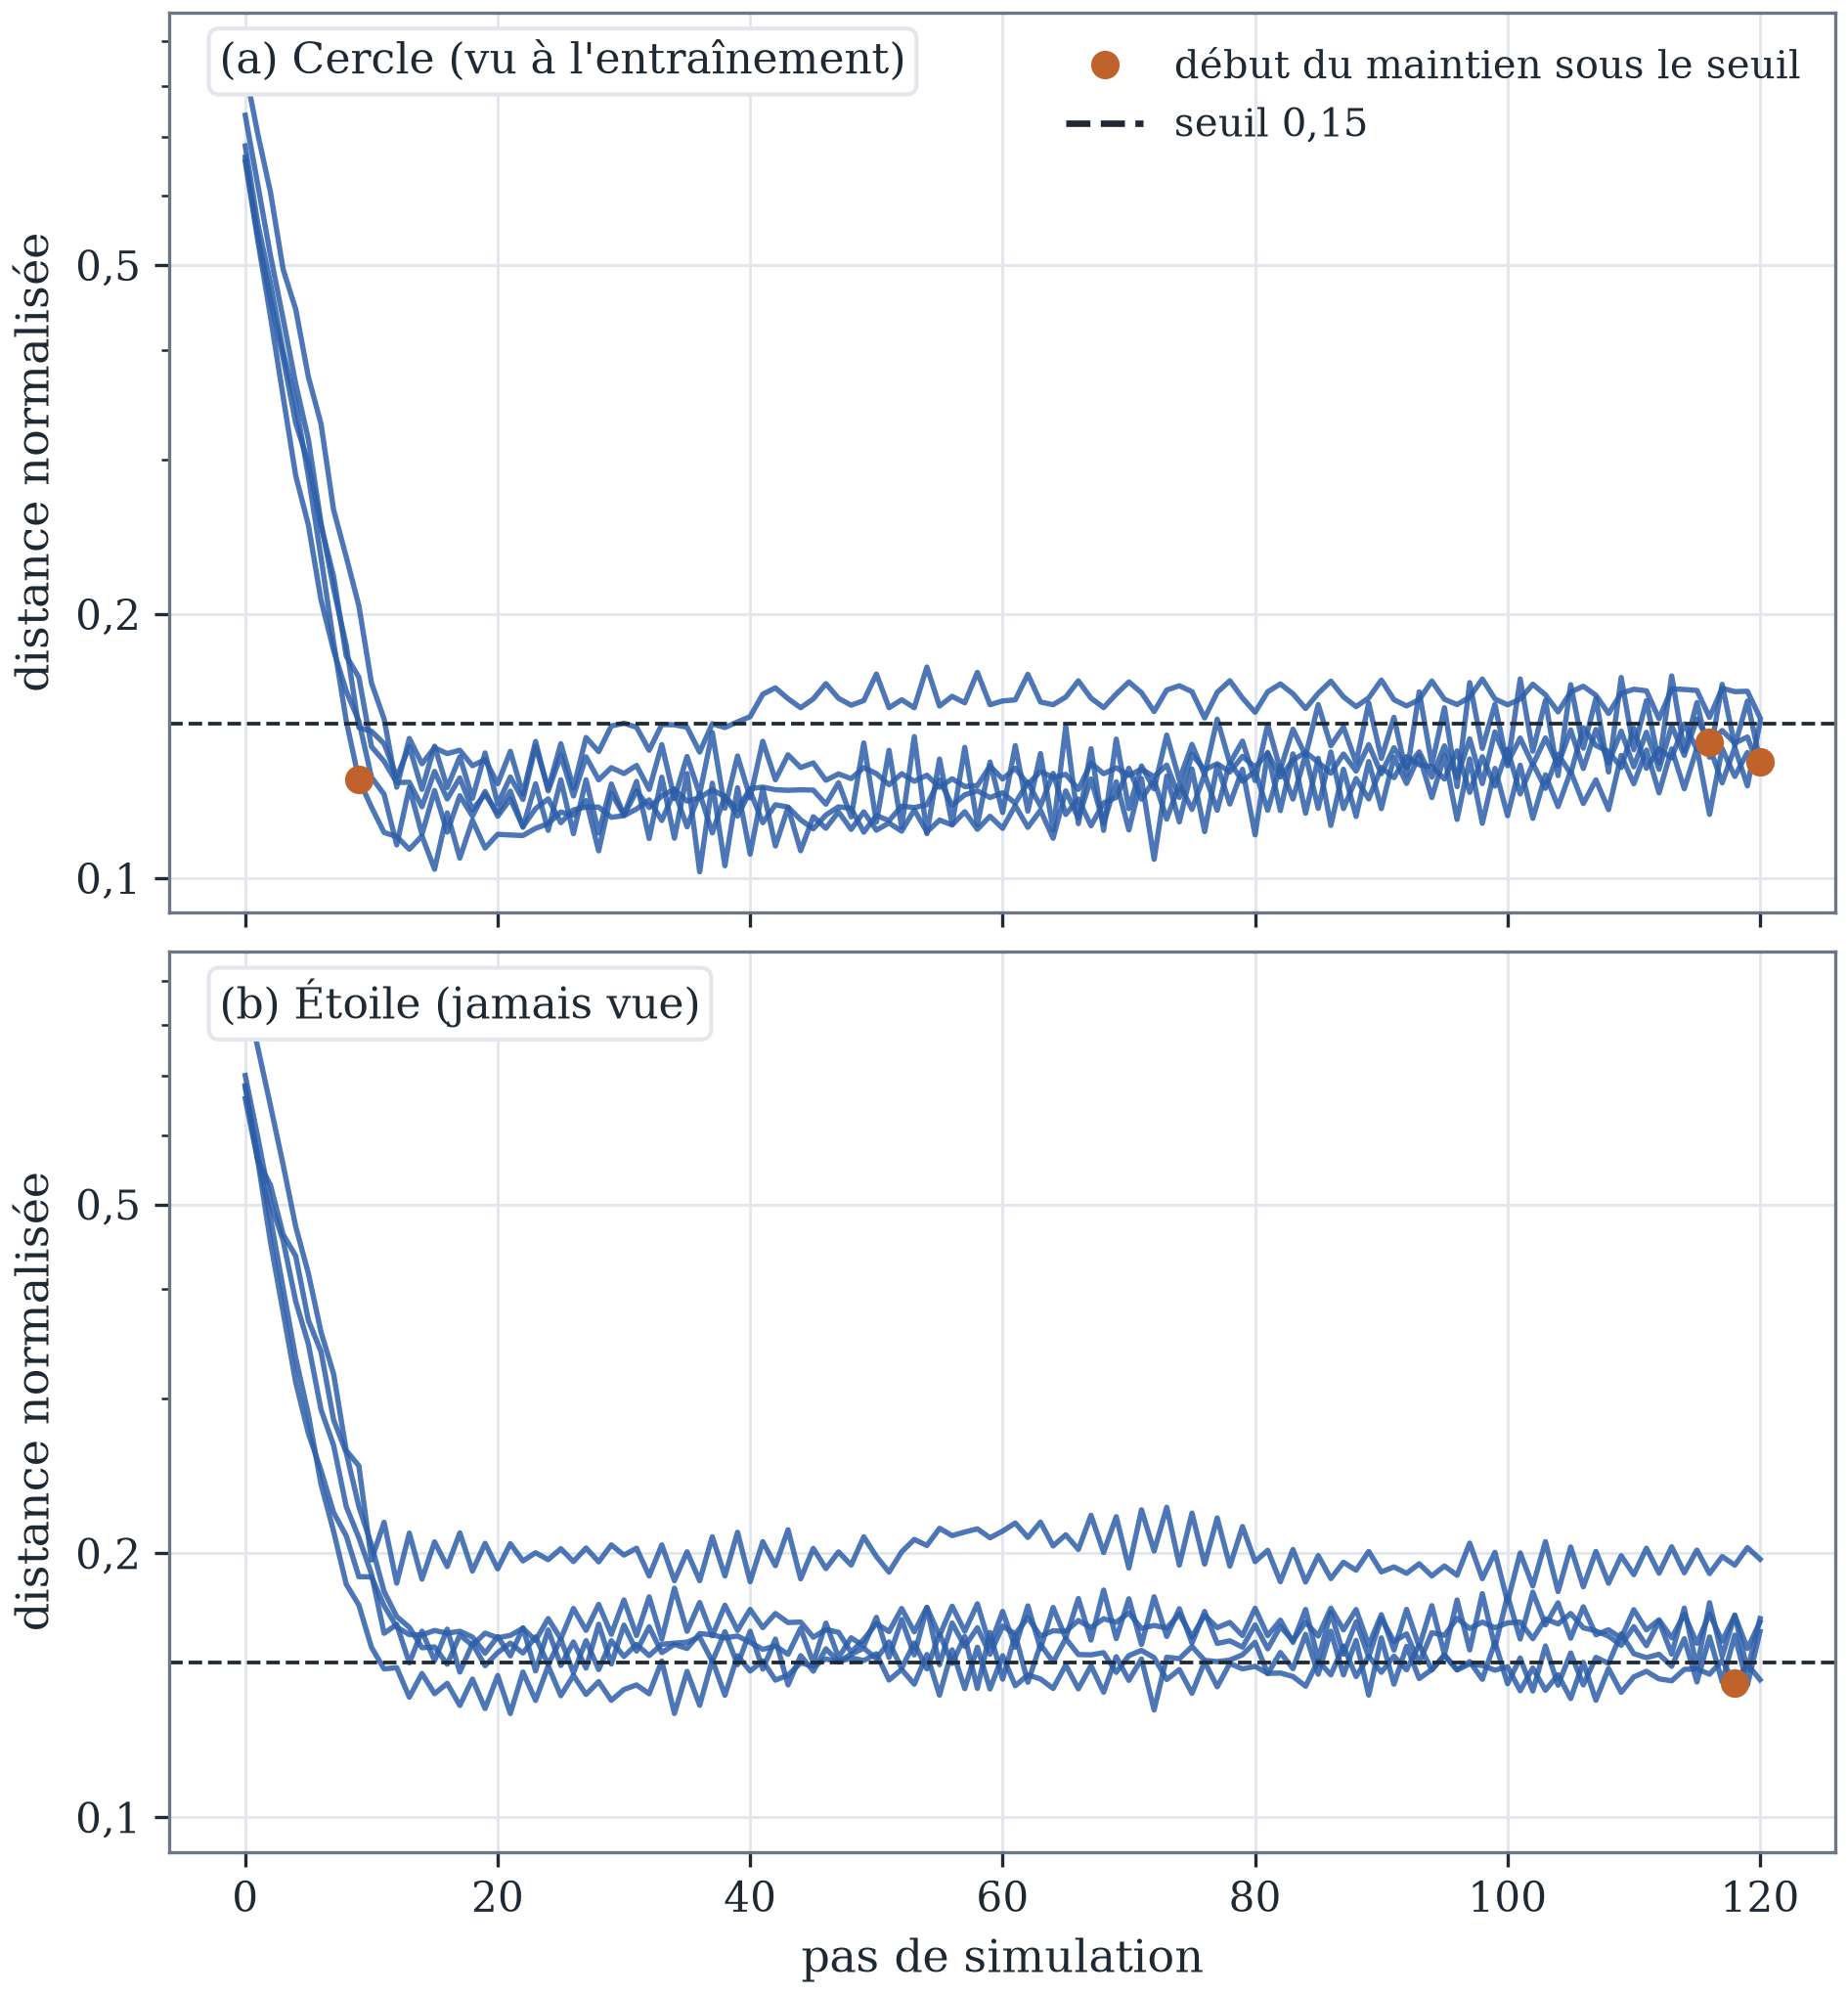
\includegraphics[width=\linewidth,height=.82\textheight,keepaspectratio]{images/real_success_criterion.png}
  \caption[Critère de succès sur des épisodes réels]{Distance au fil des pas pour cinq épisodes réels du GNN à trois tours (40 robots, graines 555000 à 555004). Le point marque le début du maintien sous le seuil 0,15. Courbes recalculées à partir des positions enregistrées.}
  \label{fig:success-criterion}
\end{figure}

\subsection{Collisions, régularité et connectivité}

Le taux de collisions rapporte le nombre de paires actives à distance inférieure ou égale à 0,1 au nombre total de paires actives disponibles sur les pas considérés. L'implémentation évalue les états qui précèdent chaque commande et laisse de côté l'état final, à la différence de la perte de collisions. C'est une fréquence de proximité dangereuse, pas un décompte d'impacts mécaniques. Retirer des robots change à la fois les paires observées et le dénominateur.

La régularité est l'écart-type des distances au plus proche voisin entre robots actifs, à l'état final. Sa version normalisée prend par défaut l'espacement du cercle unité, $2\pi/N$, et non le périmètre propre à chaque lettre ou nombre. Rappel utile dès qu'on compare des formes entre elles. Une valeur faible traduit des espacements homogènes. Elle ne montre pas que les robots couvrent la bonne cible.

Pour la connectivité, on recalcule le graphe à partir des positions enregistrées et on compte ses composantes connexes parmi les robots actifs. Un robot isolé forme une composante à lui seul. Trajectoires, masques actifs, cibles et rayons sont sauvegardés : on peut donc recalculer les mesures sans toucher aux poids.

\subsection{Comparaisons et lisibilité}

La campagne d'évaluation croise les tailles 20, 40 et 100 avec quatre fractions de retrait, de 0 à 20\,\%. Chaque condition est répétée 50 fois, et chaque variante apprise prévoit cinq graines d'entraînement. Les comparaisons appariées partagent les mêmes graines d'épisode. La variabilité entre entraînements est rapportée à part de celle entre épisodes, et les intervalles de confiance entre graines utilisent la loi de Student : avec cinq graines, le facteur vaut 2,776, et non 1,96. Réutiliser les mêmes départs sur plusieurs formes ne donne pas autant d'échantillons indépendants en plus.

Les modules disponibles prévoient la comparaison avec et sans communication, le transfert de taille à poids gelés, les formes réservées, la réduction de portée et le bruit d'observation. Ce bruit perturbe ce que reçoit le contrôleur, pas les positions physiques qui servent à mesurer la trajectoire. Ces protocoles sont implémentés, et leurs résultats restent à produire.

Pour les caractères, être géométriquement proche d'une forme ne revient pas à la faire reconnaître. Un questionnaire en aveugle sépare les images présentées de l'identité attendue, conservée dans une vérité terrain privée. Aucune réponse n'a encore été recueillie, et aucun score de lisibilité n'est donc avancé. Quand elles le seront, une matrice de confusion entre figures montrées et figures reconnues dira quelles formes se confondent, le O et le 0 par exemple.

\section{Organisation logicielle et niveau de preuve}

Les responsabilités restent séparées entre formes, simulateur, modèle, entraînement, métriques, évaluation et restitution. Chaque module lit des fichiers et en écrit d'autres. Aucun ne dépend d'un objet gardé en mémoire par un autre, si bien qu'une étude peut être rejouée sans relancer ce qui la précède.

Chaque expérience doit s'accompagner de sa configuration effective, de ses graines, de ses cibles et de la version du programme. Les campagnes chargent les poids avec leur configuration sauvegardée, vérifient la cohérence des modèles et refusent les ensembles de résultats incomplets. Un mode explicite autorise malgré tout un bilan partiel, à la condition d'en consigner chaque exclusion avec sa raison. Les rapports se construisent à partir des fichiers enregistrés, sans chiffres recopiés à la main et sans relancer d'optimisation. La reproductibilité reste conditionnelle. Elle dépend de la version, des dépendances et des données, et une même graine ne garantit pas les mêmes trajectoires d'une implémentation à l'autre.

Les tests vérifient les propriétés de permutation, de translation (sous leurs hypothèses), de bornage, de voisinage, de cibles distinctes et de cohérence des mesures. Les tests de gradient et d'orchestration simulée contrôlent la chaîne de traitement. Aucun ne montre que l'entraînement produit une politique utile. Quatre niveaux de preuve sont donc à tenir séparés : le composant implémenté, la propriété testée, le modèle réellement entraîné et la qualité mesurée sur une campagne d'évaluation.

Pour la démonstration locale, on choisit une figure, un contrôleur, un nombre de robots et une graine. Le serveur calcule l'épisode ; le navigateur affiche la trajectoire, la courbe de distance et les métriques, sans jamais exécuter de règle de contrôle. Un panneau indique pour chaque contrôleur s'il est disponible et, sinon, pourquoi. Une animation reste une illustration : l'argument scientifique du mémoire n'en dépend pas.

Reste le coût de calcul. La représentation matricielle des messages calcule toutes les paires avant le masquage. La mémoire et le temps de calcul croissent donc comme le carré du nombre de robots, même si l'agrégation reste locale. S'y ajoute le déroulement temporel, qui conserve les opérations de chaque épisode jusqu'à la rétropropagation. Les épisodes d'un lot s'exécutent l'un après l'autre, avec accumulation des pertes, au lieu d'une unique dynamique vectorisée. Les journaux donnent l'ordre de grandeur. Un entraînement de 1\,200 itérations à 40 robots a pris entre 53 et 65 minutes pour le GNN sans communication, et deux heures pour le GNN à trois tours, sur un processeur de bureau.

\section{Conclusion partielle}

Nous avons décrit la méthode à partir de ce qui est réellement implémenté : des figures décrites par des points de référence distincts et normalisés, une consigne de mission explicite, un GNN avec connexions résiduelles et une sortie bornée en norme. S'y ajoutent deux termes de forme tenus séparés, la proximité et la couverture, un apprentissage à travers une simulation différentiable par morceaux et une sélection du modèle sur validation. Les mesures et les comparaisons prévues complètent le tableau, avec une règle constante : un test logiciel réussi ne dit rien de la qualité d'un modèle entraîné. Le chapitre~\ref{chap:experiences} présente ce que cette implémentation a réellement produit : une campagne pilote de 9\,600 épisodes, ses résultats et les défauts qu'elle a permis de corriger.